\subsection{Frontend Implementering}

Det endelige design af vinderne følger tæte det oprindelige mockup design. Der benyttes MVVM (Model View View Model) designpatterns  Det har undervejs i implementeringen vist sig et behov for væsentlig flere menuer end først antaget, og disse er implementeret efter samme ovreordnede design som resten af systemet.\\
Det endelige design har følgende views: Login, Register, Main, Settings, Ingame, Load, Save, Inventory, Character, Victory, Defeat, Room og Combat.\\
Til at skifte view uden at oprætte et nyt vindue bruges et mediator design, hvor hver knap som skal skifte view notifier mediatoren. Dette virker fordi alle views er oprættet som WPF user controlls, og ikke views, hvilket tillader at et main view kan skifte mellem viewmodels. \footcite{https://www.technical-recipes.com/2018/navigating-between-views-in-wpf-mvvm/}\\

\noindent Der er implementeret at nogle af spillets funktioner kan tilgås via key-bindings, hvilket har nødsaget et brud på MVVM designet. Når mediatoren skifter view bilver fokus ikke sat til det nye view, og keybinding virker derfor ikke. For at løse dette sættes top-elementet på den nye side som fokus. Dette kan dog ikke gøres i MVVM, så her er det pattern brudt, da det er nødvændigt at gå ind i code-behind filen for at sætte fokus.

\noindent De følgende afsnit viser et udvalg af view, samt en beskrivelse af hvordan de afviger fra det oprindelige design og en beskrivelse af interesante programerings-tekniske beslutninger.

\subsubsection{Login view}
De overordnede struktur af login (\autoref{fig:Design-FE-impl-login}) og register menuerne følger meget tæt det oprindelige design. Alle elementer er blevet stiliseret så de matcher det ønskede look. Dette er gjort ved brug af globale resourses og styles i app.xaml filen. Dette gør det nemt at oprætte nye views og ændre udseende af hele spillet. Selve login håndteres af backenden som kaldes af login og register knapperne via command binding.

\begin{figure}[h]
\centering
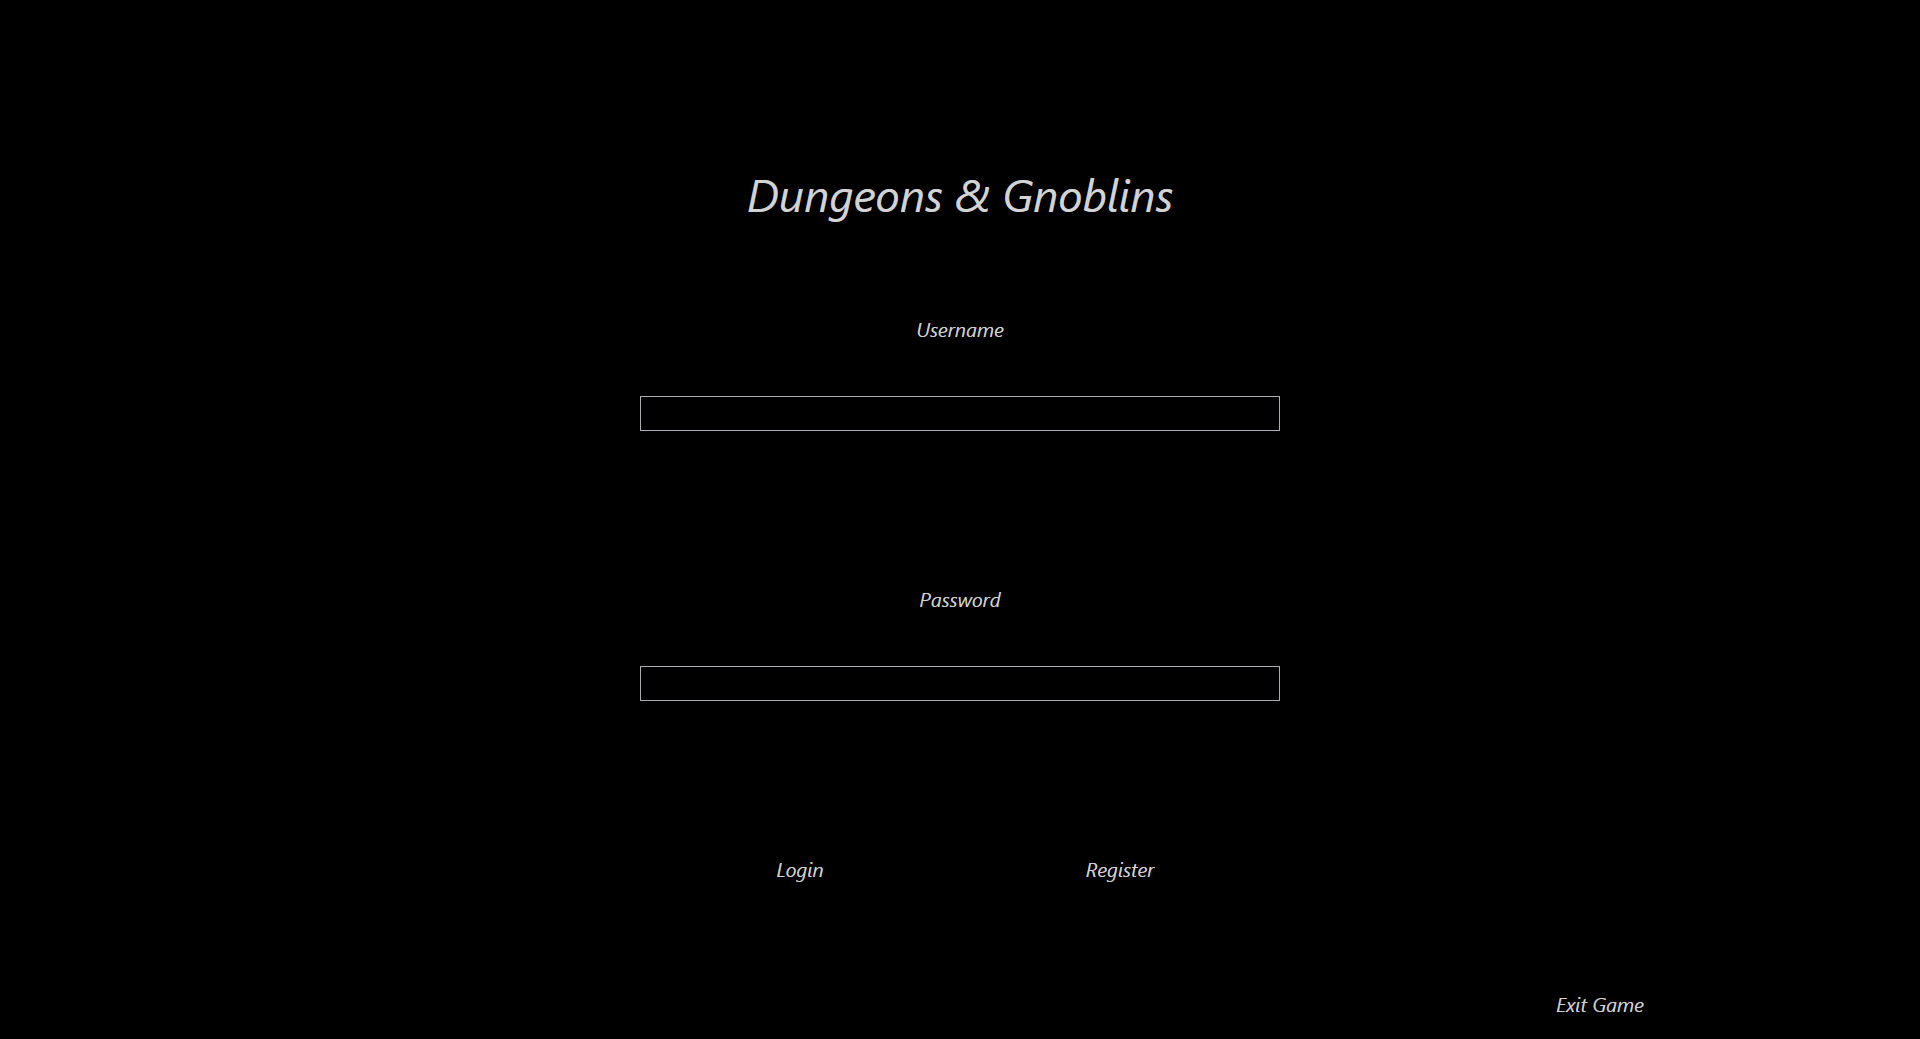
\includegraphics[width = \textwidth]{02-Body/Images/login_final.PNG}
\caption{Endelig login skærm. Brugenav og kodeord kan indtastes i de to felter.}
\label{fig:Design-FE-impl-login}
\end{figure}

\subsubsection{Room View}

Visuelt er room view (\autoref{fig:Design-FE-impl-room}) ikke ændret betydeligt fra det oprindelige design. Der er ændret lidt på placering og antal af knapper så det passer til antallet af interaktioner tilgængelig til brugeren. Kortet er lavet så det  opdateres når spilleren går ind i et nyt rum, ved at ændre på synligheden af elementerne i kortet. Det er yderligere sat op så det kan skaleres til de skærmopløsninger som understøtes.\\
Ved at trykke på interact knappen kan spilleren flytte et valgt 'item' fra listennederst til venstre over i sit inventory (et seperat view), som kan tilgås veed at trykke på Inventory knappen.\\
Alt tekst er vist med data binding.

\begin{figure}[h]
\centering
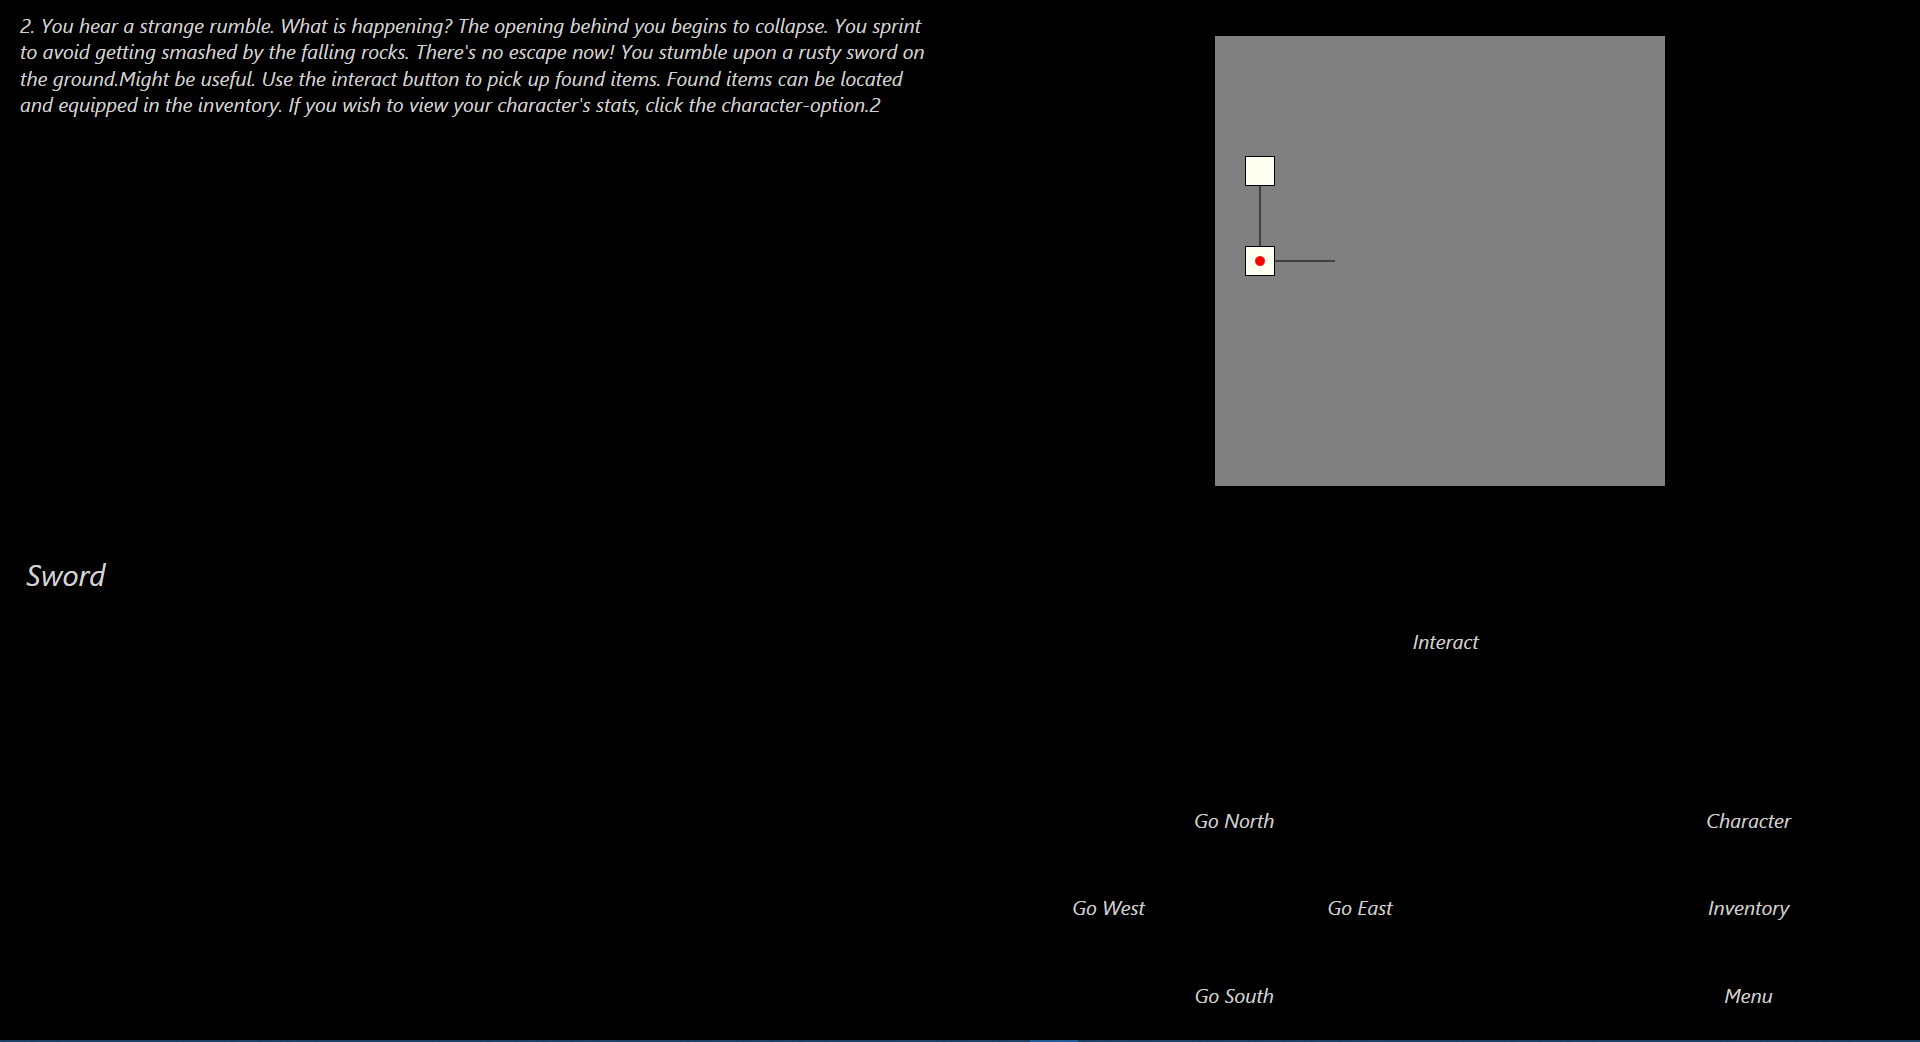
\includegraphics[width = \textwidth]{02-Body/Images/room_final.PNG}
\caption{}
\label{fig:Design-FE-impl-room}
\end{figure}

\subsubsection{Combat View}

Combat view (\autoref{fig:Design-FE-impl-combat}) er bygget med room view som skabelon, så de fleste elementer er ens. Knappernes antal og funktion er ændret, og samenlignet med det oprindelige design er knapperne for items og character fjernet, da det blev besluttet at det ikke skulle være muligt at tilgå sit inventory under en kamp. I stedet for en beskrivelse af rummet og en liste af items vises der nu en beskrivelse af hvordan kampen går i venstre side af skærmen. Tal værdierne hentes fra gameengine, og sættes ind i en tekststreng som gør det nemt at forstå hvordan det skal fortolkes. Der er yderligere tilføjet en healthbar, som giver en visuel indikation af hvor tæt spilleren er på at tabe spillet og skifter frave fra grøn til gul til rød efter som spilleren tager mere skade. Baren giver derfor lidt frave til et ellers meget gråtonet spil.

\begin{figure}[h]
\centering
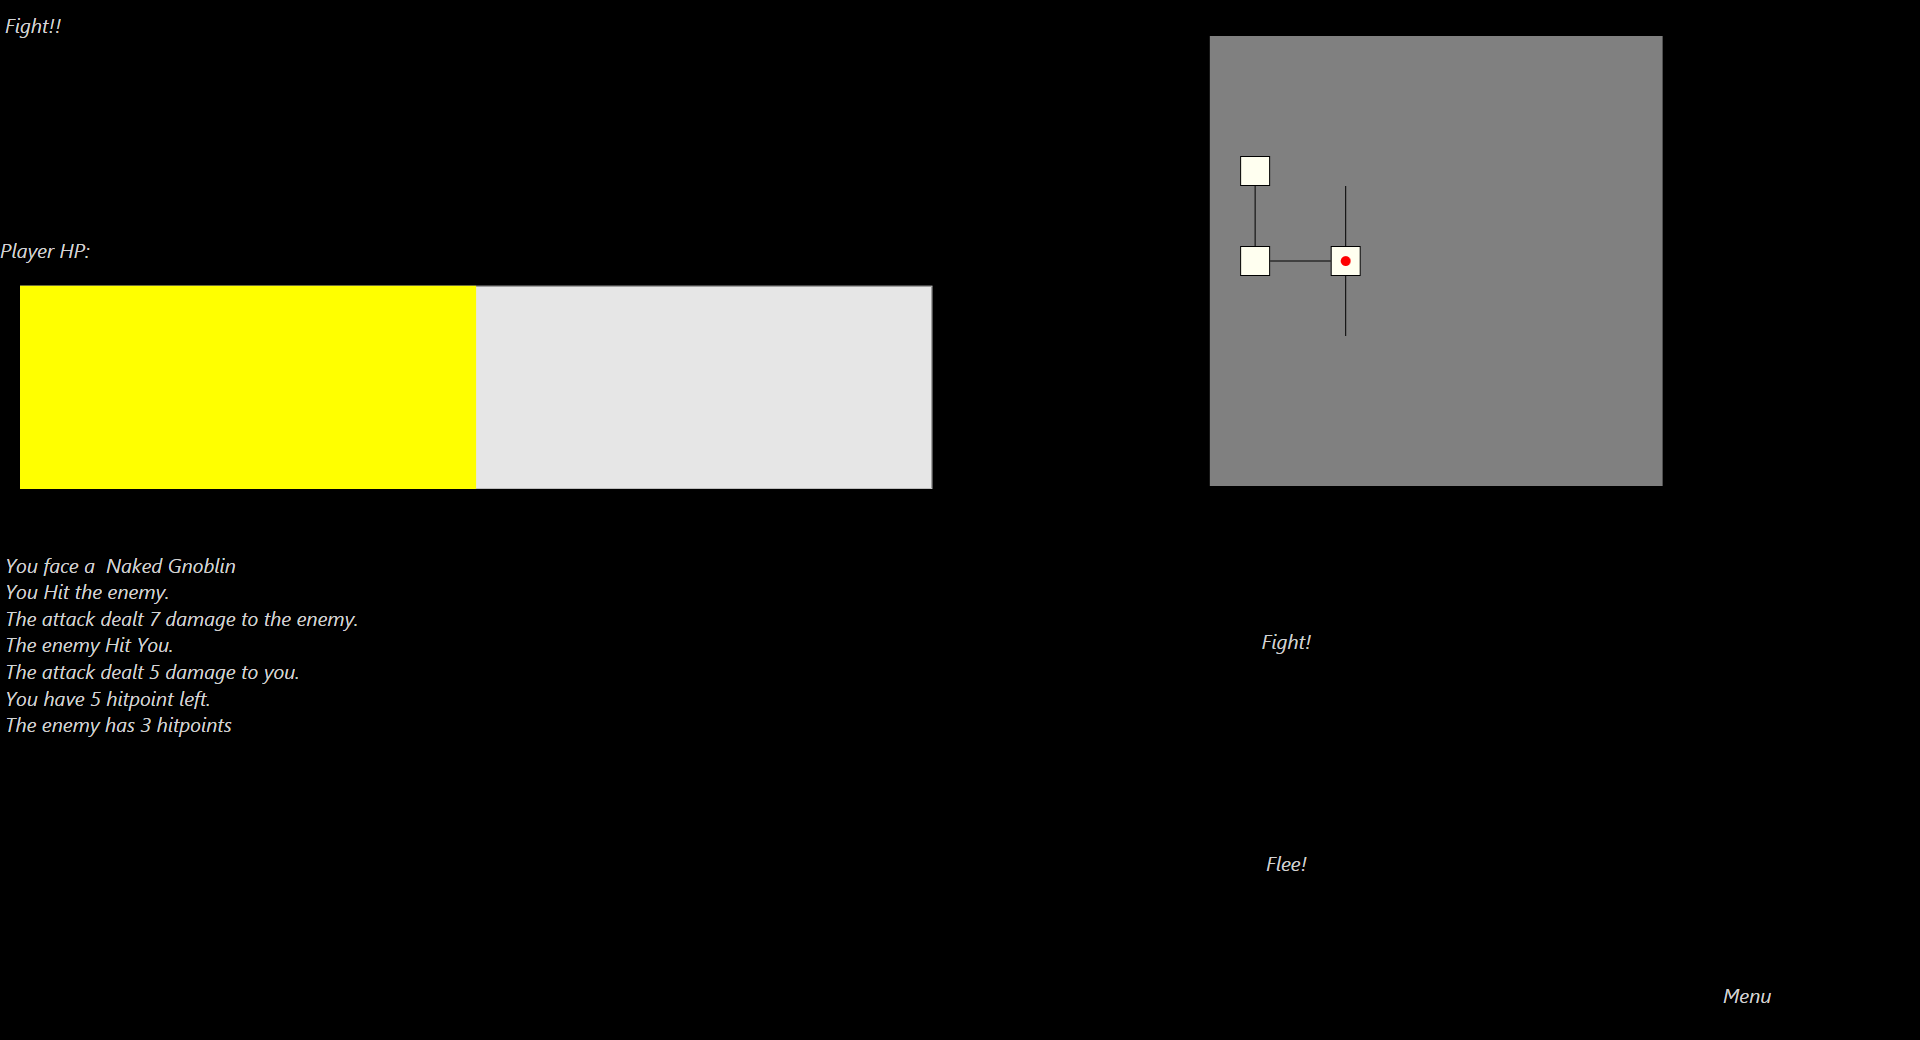
\includegraphics[width = \textwidth]{02-Body/Images/combat_final.PNG}
\caption{}
\label{fig:Design-FE-impl-combat}
\end{figure}

\subsubsection{Settings view}

I settingsmenuen (\autoref{fig:Design-FE-impl-settings}) er det muligt at vælge lydstyrke for musikken i spillet (samt slukke helt for musikken) og vælge mellem tre skærmopløsninger (720x480, 1920x1080 og 2k). Det tre valgmuligheder er valgt til at teksten på skærmen stadig er læselige. Kortet i Room og Combat view skalerer med skærmopløsningen, men sætter en nedre grænse på 300x300 pixel. Tekststørelsen gør dog at den praktiske nedre grænse, hvor spillet ser ud som det skal, er 720x480. Ved skærm opløsning større end 2k bliver teksten og kortet for småt til at kunne ses ordentligt, hvorfor 2k er en naturlig øvre grænse for skærmopløsningen. Alle opløsninger imellem de to grænser burde være i orden (så længe det bare nogenlunde følger en 4:3 eller 16:9 ratio).\\

\noindent For at sørge for at den valgte skærmopløsning er brugt i alle views er der oprættet et objekt til at holde indstillings informationer, samt andre info som det ønskes at kunne tilgå fra flere forskællige views. Denne klasse følger et singleton design pattern, og den samme instance af objektet kan derfor tilgås fra alle de view som skal bruge informationer derfra.\\

\noindent
Settings menuen kan tilgås fra både main menu og ingame menu, og det er derfor nødvændigt at spillet ved hvilken menu man var i inden man gik ind i settings menuen, så spillet kan gå tilbage til den rigtige menu når der trykkes på back. Til dette bruges singleton objektet også, da det gør det nemt at bringe informationen mellem views. Dette bruges også i ingame menu, da denne kan tilgås fra både room view og combat view.

\begin{figure}[h]
\centering
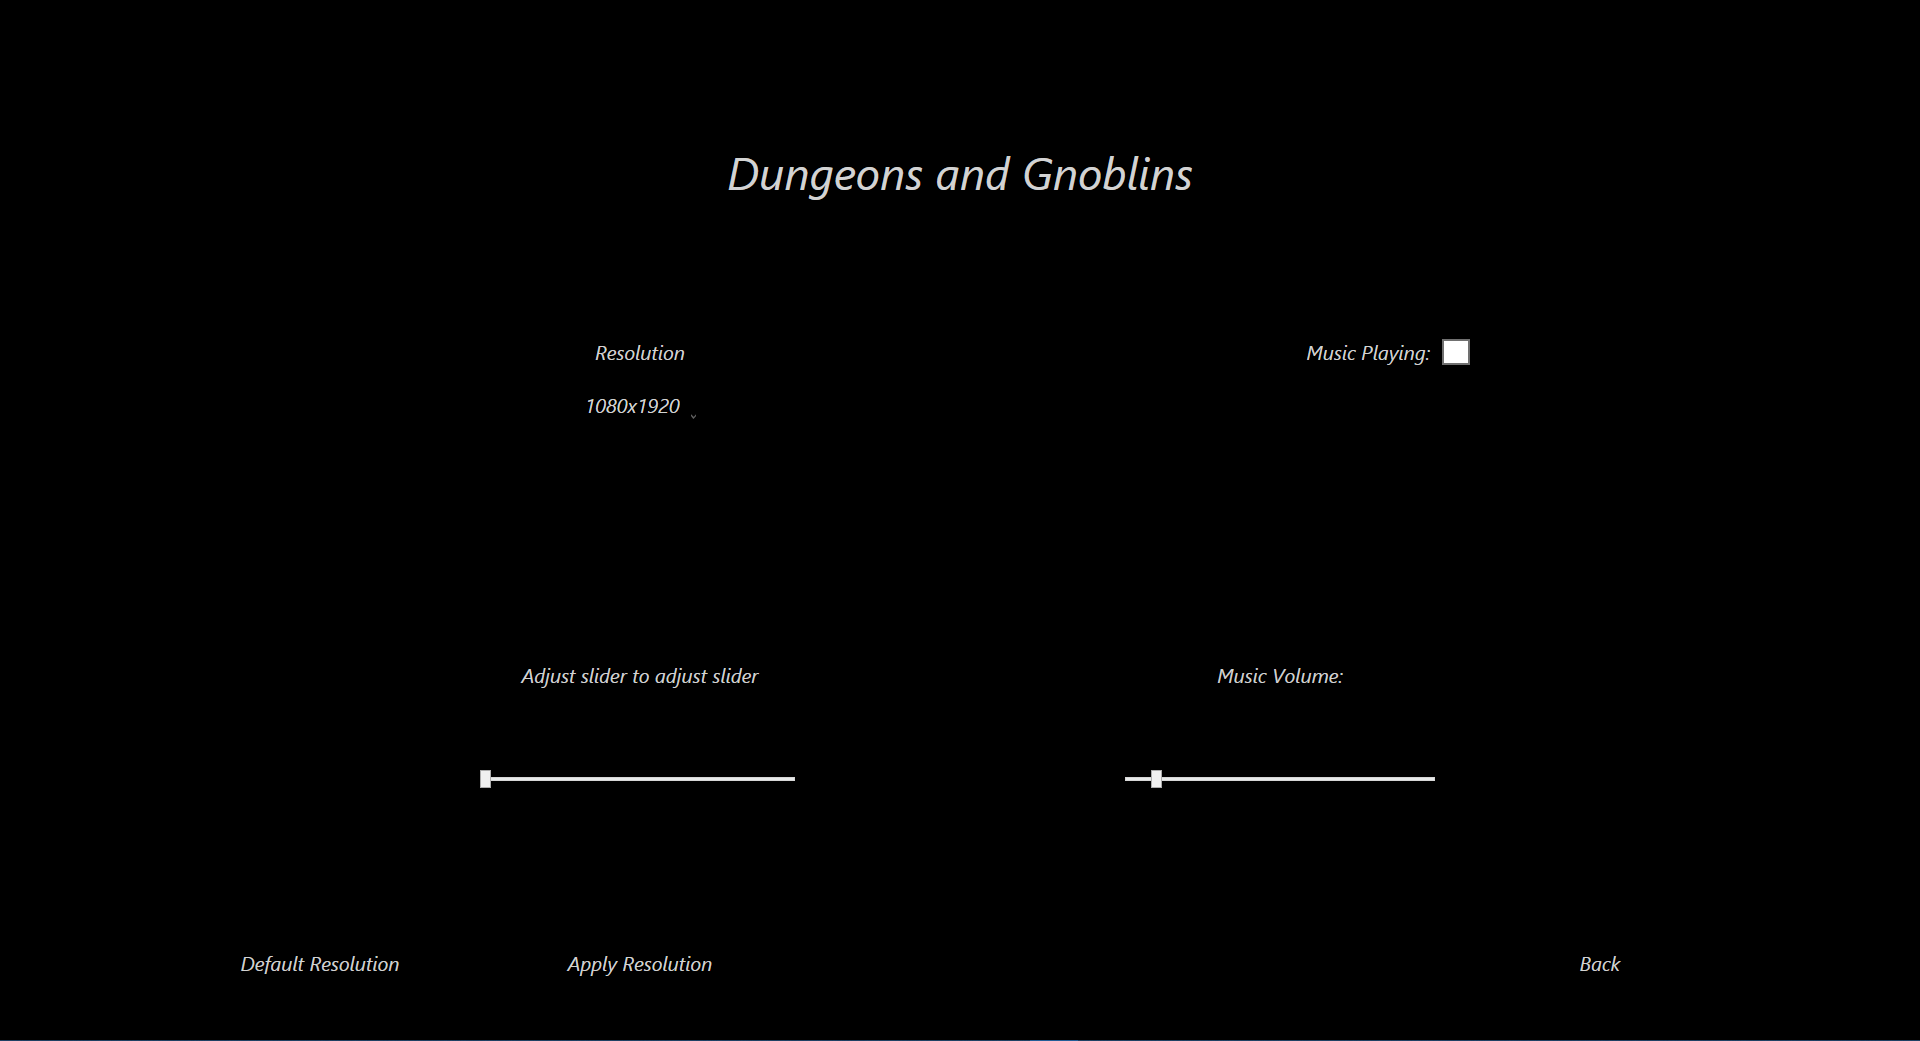
\includegraphics[width = \textwidth]{02-Body/Images/SettingsMenu_final.PNG}
\caption{}
\label{fig:Design-FE-impl-settings}
\end{figure}

\subsubsection{Load view}

Load (\autoref{fig:Design-FE-impl-load}) og Save menuerne præsenterer spilleren med en liste af gemte spil, som brugeren kan hente, eller gemme. Dette opnås ved at der hver gang spilleren åbner en af de to menuer, hentes en liste af tilgængelige 'save-games', som via databinding, præcenteres for brugeren. Når der trykkes på Save/Load sendes den fornødne kommando til backenden.

\begin{figure}[h]
\centering
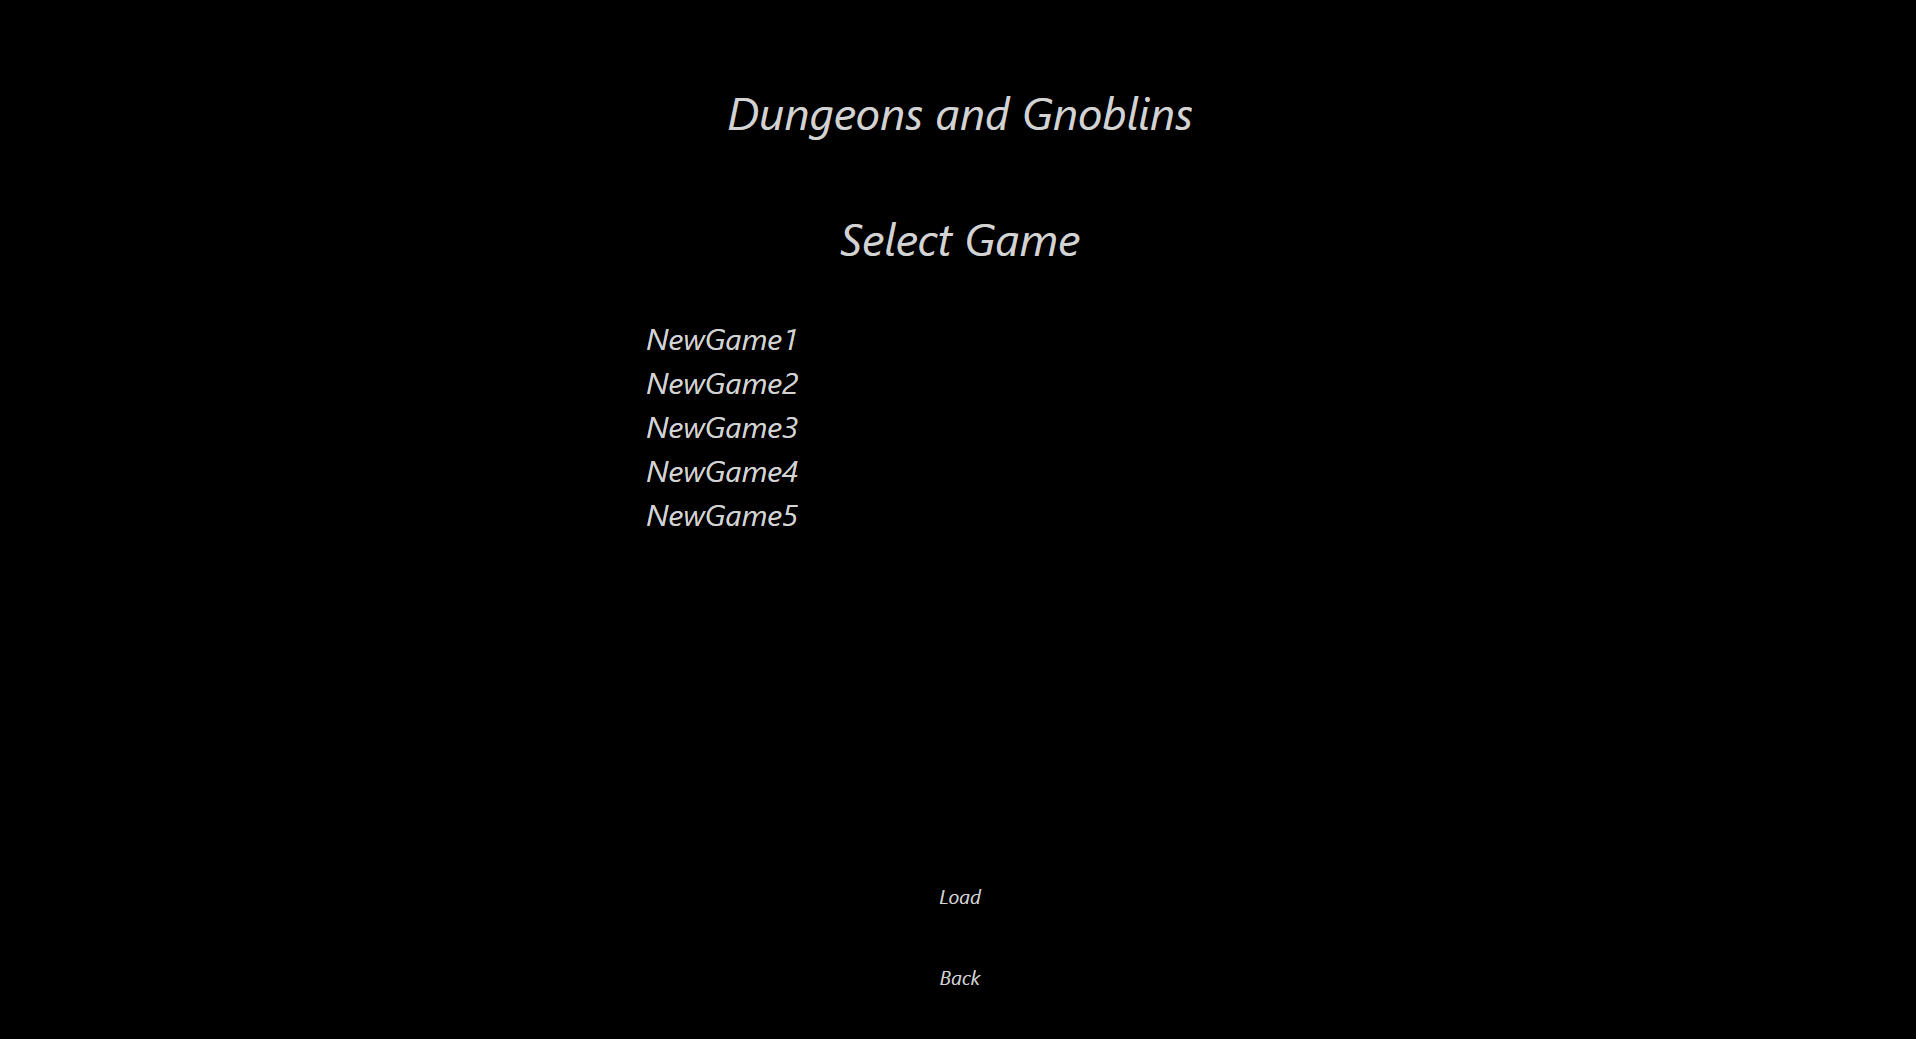
\includegraphics[width = \textwidth]{02-Body/Images/LoadMenu_final.png}
\caption{}
\label{fig:Design-FE-impl-load}
\end{figure}

\subsubsection{Note om Baggrundsfarver}
Da den generalle baggrundsfarve i spillet er sort er alle spillets interface ellementer oprættet så baggrundsfarven matcher. Dette er for det meste nemt opnået ved brug at WPF styles, men enkelte elementer (så som resolution dropdown menu) viste sig at være betydeligt mere omfattende. Det viser sig at det valgte element (WPF combobox) ikke tillader at baggrundsfarven for dropdown elementerne ændres i Windows 8 eller senere. . Løsningen er at lave en kopi af hele templaten (ca. 300 linjer kode) for combobox og ændre 3-4 linjer. \footcite{https://social.technet.microsoft.com/wiki/contents/articles/24240.changing-the-background-color-of-a-combobox-in-wpf-on-windows-8.aspx}

\newpage
